\part{Contribution}

\chapter{Organisme d’accueil}

\section{Introduction}
Dans ce chapitre, nous présenterons l’organisme qui nous a accueillis pour la
réalisation de notre projet de fin d’études. Nous commencerons par une brève
introduction de l’entreprise, en mettant en évidence son domaine d’activité et
son positionnement sur le marché. Ensuite, nous détaillerons les différents
services proposés par l’organisme, ainsi que son organigramme organisationnel.
Cette présentation nous permettra de mieux comprendre l’environnement dans
lequel notre projet s’est déroulé et les contraintes spécifiques auxquelles
nous avons été confrontés.

\section{Présentation de l'organisme d'accueil}
STIE, ou Schneider Toshiba Inverter Europe SAS, est un département relié à
Schneider Electric. Ce département offre une gamme complète d'équipements
électroniques industriels. Il propose des inverseurs polyvalents, des
variateurs de vitesse industriels, des composants de contrôle, et des produits
de distribution électrique. STIE dispose également de laboratoires équipés de
divers matériels, tels que des moteurs électriques et leurs dérivés, pour
répondre aux besoins de ses clients à travers le monde. STIE est principalement
basé à Pacy-sur-Eure.

\textbf{Schneider Electric} est un leader mondial de la technologie industrielle
avec une expertise de référence dans l'électrification,l'automatisation, et la
digitalisation des industries intelligentes, des infrastructures résilientes, des
centres de données durables, des bâtiments intelligents, et des maisons intuitives.
L'entreprise mène la transformation numérique de la gestion de l'énergie et des
automatismes dans les secteurs résidentiel, des bâtiments, des centres de données,
des infrastructures et des industries.
Présente dans plus de 115 pays, Schneider Electric est le leader incontesté de la
gestion électrique, couvrant la moyenne tension, la basse tension, l'énergie sécurisée, et
les systèmes d'automatismes. La société fournit des solutions d'efficacité intégrées qui
associent gestion de l'énergie, automatismes, et logiciels. L'écosystème qu'elle a construi
t lui permet de collaborer sur sa plateforme ouverte avec une large communauté de partenaires,
d'intégrateurs, et de développeurs pour offrir à ses clients à la fois contrôle et efficacité
opérationnelle en temps réel. Son siège social est situé à Rueil-Malmaison,
et la répartition géographique de son chiffre d'affaires est la suivante :

\begin{itemize}
  \item France : 5,8\%
  \item Europe de l'Ouest : 18,5\%
  \item États-Unis : 27,9\%
  \item Amérique du Nord : 4,2\%
  \item Chine : 15,1\%
  \item Asie-Pacifique : 15,2\%
  \item Autres : 13,3\%
\end{itemize}

\section{Services}

Schneider Electric propose une gamme étendue de produits et services innovants,
notamment :
\begin{itemize}
  \item \textbf{Produits d'automatisation et de contrôle} : Solutions complètes pour l'automatisation des processus et la gestion des systèmes de contrôle industriel.
  \item \textbf{Produits et systèmes basse tension} : Équipements pour la distribution électrique et la protection des installations basse tension.
  \item \textbf{Énergie solaire et stockage} : Solutions pour la production d'énergie solaire et le stockage d'énergie.
  \item \textbf{Distribution moyenne tension et automatisation du réseau} : Systèmes pour la distribution d'énergie moyenne tension et l'automatisation des réseaux électriques.
  \item \textbf{Énergie critique, refroidissement et racks} : Solutions pour la gestion de l'énergie critique, le refroidissement des infrastructures et les racks de serveur.
\end{itemize}

\section{L’organigramme de Schneider Electric}

L'organigramme de Schneider Electric représente la structure de l’entreprise et
les relations hiérarchiques entre ses membres. Voici une description détaillée
de la structure organisationnelle de Schneider Electric :

\textbf{Direction Générale}

À la tête de l’entreprise se trouve Peter Herweck, PDG. Il est responsable de la direction générale et de la prise de décisions stratégiques.

\textbf{Équipe de Management}

L'équipe de direction de Schneider Electric comprend plusieurs membres clés.
Peter Herweck occupe le poste de PDG, apportant une vision stratégique globale
à l'entreprise. Barbara Frie est responsable de la Proposition de Valeur
Employé, tandis que Deepu Chawla occupe le poste de Vice-Président Senior.
Chaque membre apporte une expertise unique et une vision stratégique à
l'entreprise.

\textbf{Département des Ressources Humaines}

Le département des ressources humaines est supervisé par Perrine Colson,
Partenaire Commerciale en Ressources Humaines. Elle est responsable de la
gestion du personnel, du recrutement et de l'administration du personnel..

\textbf{Département de R\&D}

Le département de Recherche et Développement (STIE) est dirigé par Allan
Pierre, Directeur de la R\&D globale. Il est responsable de l'innovation, de la
conception, de l'évolution et de la maintenance des Variateurs de Vitesse et
Démarreurs Progressifs chez Schneider Electric. Allan Pierre gère une équipe de
plus de 300 professionnels, assurant l'alignement avec les objectifs
stratégiques et les exigences des clients.

\textbf{Équipe de Drive R\&D}

L’équipe de Drive R\&D se concentre sur la recherche et le développement dans
le domaine des drives, la partie qui contrôle les moteurs électriques. Cette
équipe est dirigée par Al Kassem Jebia, avec des membres clés tels que Nicolas
Henwood et Ali Tfaily avec qui je travaille, cette équipe contribue à
l'avancement des technologies et des solutions innovantes pour les moteurs
électriques.

\section{Conclusion}
Dans ce chapitre, nous avons présenté l’organisme d’accueil qui nous a permis
de réaliser notre projet de fin d’études. Nous avons fourni une description
détaillée de l’entreprise, de ses activités principales et de son
positionnement sur le marché. Nous avons également mis en évidence les
différents services proposés par l’organisme, ainsi que son organigramme
organisationnel.

Cette présentation nous a permis de mieux comprendre l’environnement dans
lequel notre projet s’est déroulé et les contraintes spécifiques auxquelles
nous avons été confrontés.

%%%%%%%%%%%%%%%%%%%%%%%%%%%%%%%%%%%%%%%%%%%%%%%%%%%%%%

\chapter{Conception}

%\newpage

\section{Introduction}

Dans ce chapitre, nous aborderons la problématique centrale à laquelle ce
projet tente de répondre ainsi que la solution proposée pour la résoudre. La
problématique identifiée concerne la nécessité de disposer d'un jeu de données
plus riche et plus diversifié, capable de couvrir une large gamme de moteurs
électriques disponibles sur le marché. Cette diversité est essentielle pour
développer des modèles de maintenance prédictive robustes et généralisables.

Pour pallier le manque de données réelles disponibles pour tous les types de
moteurs, nous proposons l'utilisation de modèles génératifs. Ces modèles
permettent de créer artificiellement des données supplémentaires, tout en
assurant que celles-ci reflètent fidèlement les caractéristiques des données
réelles. Nous présenterons en détail les modèles génératifs utilisés, ainsi que
leurs architectures.

De plus, nous discuterons des types de données que nous cherchons à générer, en
précisant l'architecture de données mise en place pour l'entraînement des
modèles génératifs. Enfin, nous présenterons les méthodes d'évaluation
employées pour mesurer la qualité des données générées, en s'assurant qu'elles
sont suffisamment représentatives des données réelles et utiles pour les
applications de maintenance prédictive.

\section{Problématique et besoins}

Dans le cadre de mon stage chez Schneider Electric, l'objectifs final est de
développer une solution de maintenance prédictive pour les moteurs électriques
asynchrones. La maintenance prédictive a pour but de détecter les défauts
potentiels avant que le moteur ne tombe en panne, en s'appuyant sur une
approche basée sur le machine learning. Cette méthode nécessite l'utilisation
d'un modèle de réseaux de neurones, qui doit être entraîné sur une grande
quantité de données afin d'être performant.

Cependant, une problématique majeure se pose : il existe une multitude de
marques et de modèles de moteurs électriques, chacun ayant des caractéristiques
différentes. Pour que la maintenance prédictive soit efficace, il est essentiel
de développer une solution qui soit généralisable à tous les types de moteurs
utilisés par les clients de Schneider Electric. Toutefois, il est pratiquement
impossible de collecter des données exhaustives sur tous les moteurs
disponibles sur le marché, ce qui complique considérablement l'entraînement du
modèle de machine learning.

Chez Schneider Electric, une des solutions techniques envisagées repose sur
l'utilisation d'un dispositif appelé "Drive" (illustré à la figure
\ref{fig:drive}). Ce drive est connecté au moteur électrique et permet de
contrôler des paramètres essentiels tels que le couple et la vitesse. De plus,
il est capable de lire les signaux entrants et sortants du moteur asynchrone
triphasé.

Le drive de Schneider est équipé d'un microcontrôleur, et l'idée est de
déployer un modèle de classification directement sur ce microcontrôleur afin de
détecter les défauts ainsi que les types de pannes dans un moteur asynchrone
triphasé. Ce modèle, embarqué sur le microcontrôleur, devra être capable de
fonctionner efficacement en temps réel pour identifier les défaillances
potentielles et alerter les opérateurs avant qu'une panne majeure ne survienne.

\begin{figure}[hbt!]
  \centering
  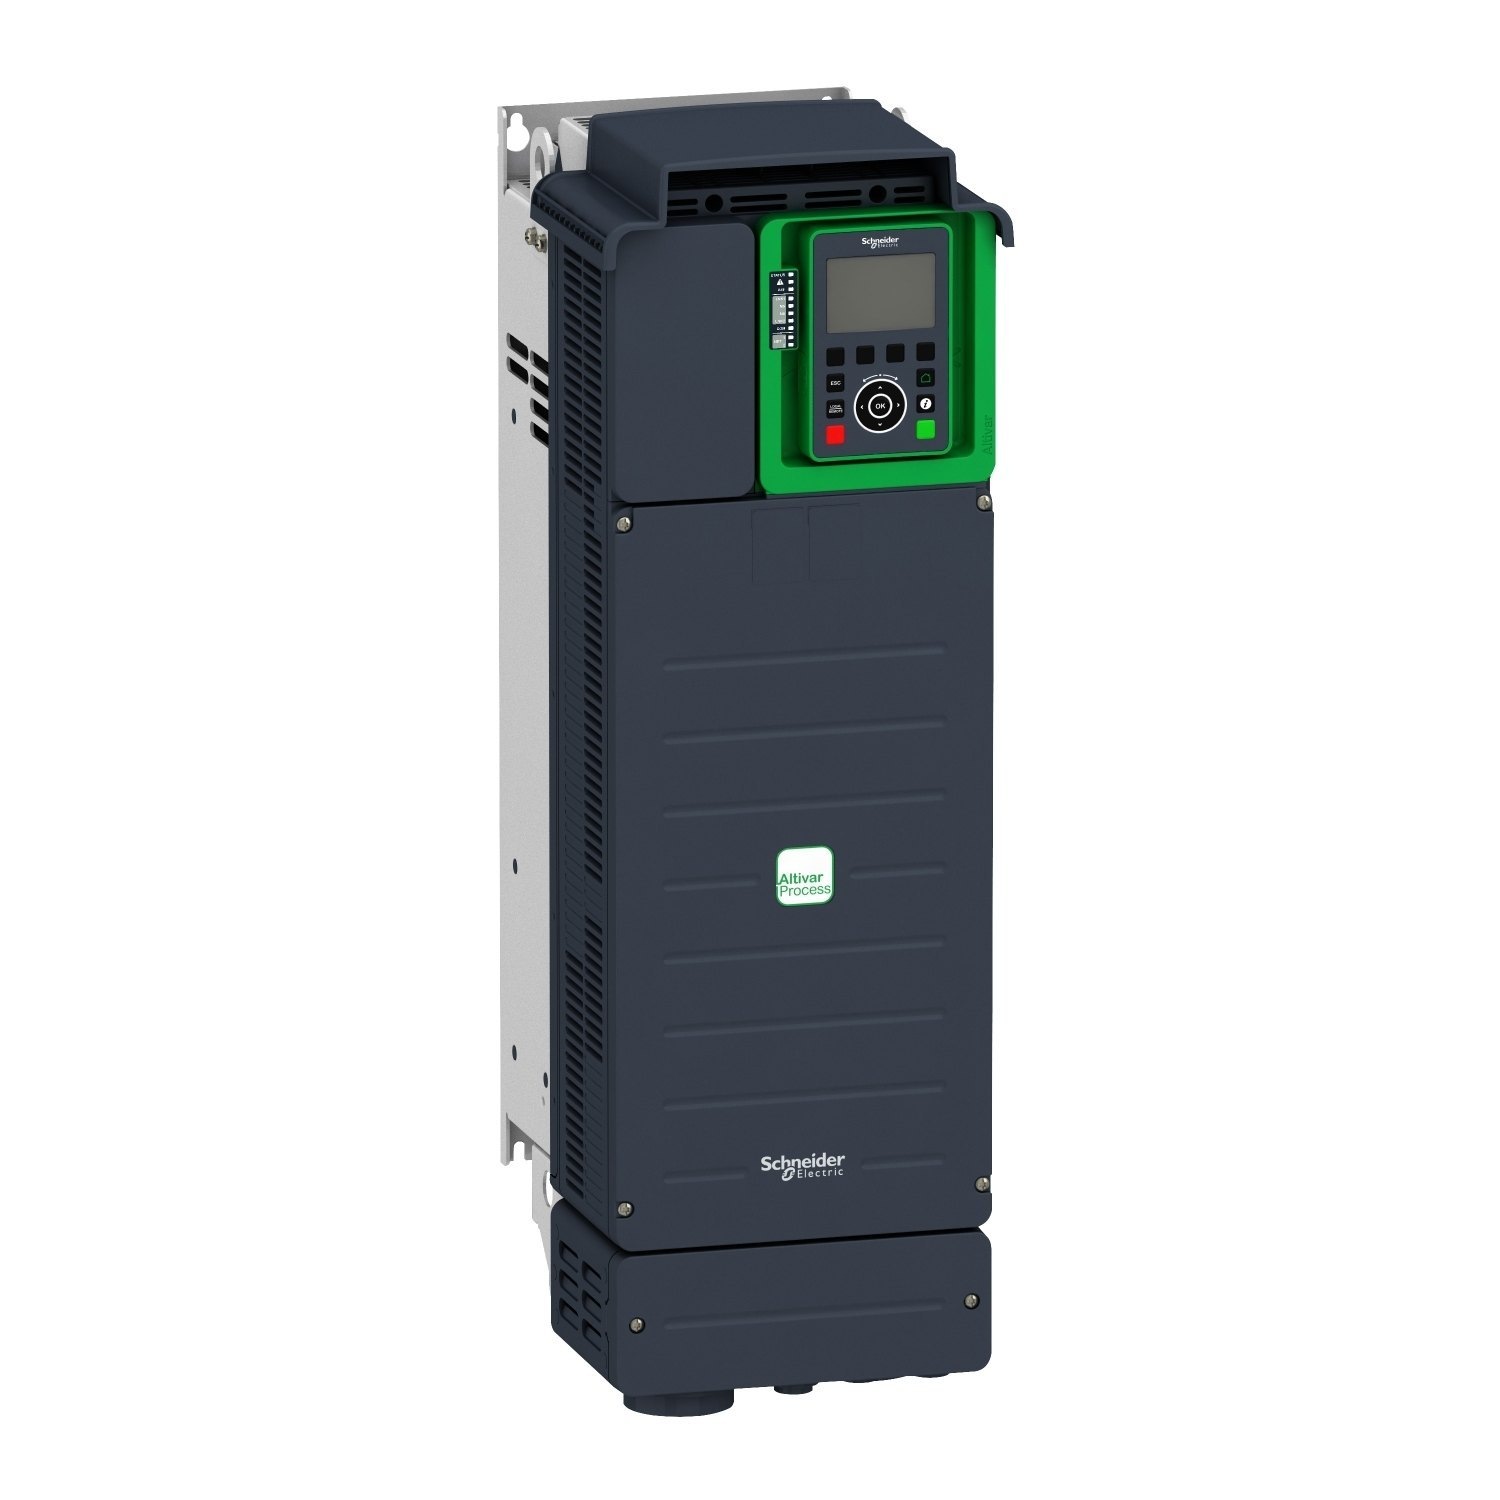
\includegraphics[width=10cm]{images_pfe/drive_se.jpg}
  \caption{Schneider Electric ATV930D30N4 AC Speed Drive.}
  \label{fig:drive}
\end{figure}
\FloatBarrier

\subsubsection{Objectifs du stage:}

\begin{itemize}
  \item Génération de données d'un moteur en bon état (healthy)
  \item Génération de données d'un moteur en mauvais état (non healthy) ayant déjà subi
        un défaut
  \item Utilisation de modèles génératifs pour la détection des défauts
\end{itemize}

La finalité de notre projet est de développer un modèle génératif capable
d'être entraîné sur les données réelles provenant de moteurs électriques. Une
fois entraîné, ce modèle pourra générer des données qui, bien qu'aléatoires,
seront similaires aux données d'origine. L'objectif est de garantir que ces
nouvelles données restent fidèles aux caractéristiques des données réelles,
tout en étant suffisamment distinctes pour éviter toute redondance exacte. Ce
processus permet de simuler des scénarios variés et d'enrichir le jeu de
données avec des exemples réalistes, sans pour autant reproduire à l'identique
les enregistrements initiaux.

\section{Notions}

\begin{itemize}

  \item \textbf{Couple et Vitesse} \\
        Le couple et la vitesse sont deux paramètres clés qui caractérisent le fonctionnement d'un moteur électrique.
        \begin{itemize}
          \item \textbf{Couple (T)} : Le couple (Torque en anglais) est la force rotative produite par le moteur, exprimée en Newton-mètre (Nm). Il représente la capacité du moteur à produire une rotation et est directement lié à la charge que le moteur peut entraîner. Le couple est un indicateur crucial de la performance d'un moteur, surtout dans des conditions de charge variable.
          \item \textbf{Vitesse (S)} : La vitesse (Speed en angalais) , généralement mesurée en tours par minute (tr/min), désigne la rapidité avec laquelle l'arbre du moteur tourne. Elle est souvent liée à la fréquence du courant alternatif dans les moteurs asynchrones, mais peut être contrôlée à l'aide de variateurs de vitesse. La relation entre le couple et la vitesse est un point central dans la caractérisation du point de fonctionnement d'un moteur.
        \end{itemize}
        \textbf{Le point de fonctionnement} d'un moteur est donc défini par une combinaison spécifique de couple et de vitesse \textbf{(} $\mathcal{T}$\textbf{orque, }$\mathcal{S}$\textbf{peed)}, et il évolue en fonction des conditions de charge et des paramètres d'alimentation du moteur. Un suivi précis de ces deux paramètres est essentiel pour la maintenance et le diagnostic des moteurs.

  \item \textbf{Glissement} \\
        Le glissement (Slip en anglais) est généralement exprimé en pourcentage. Il représente le décalage relatif  entre la vitesse de rotation du champ magnétique du stator, appelée vitesse synchrone  et la vitesse réelle du rotor, et constitue une caractéristique clé du fonctionnement des moteurs asynchrones.

        La formule du glissement (\(s\)) est donnée par \ref{equ:slip} :

        \begin{equation}
          s = \frac{N_s - N_r}{N_s} \cdot 100
          \label{equ:slip}
        \end{equation}

        où :
        \begin{itemize}
          \item \(N_s\) est la vitesse synchrone, exprimée en tours par minute (tr/min),
          \item \(N_r\) est la vitesse réelle du rotor, exprimée en tours par minute (tr/min).
        \end{itemize}

  \item \textbf{Courant et Tension} \\
        Le courant et la tension sont deux paramètres électriques fondamentaux pour le fonctionnement des moteurs électriques.
        \begin{itemize}
          \item \textbf{Courant (I)} : Le courant électrique, mesuré en ampères (A), est le flux de charges électriques à travers les enroulements du moteur. Une mesure précise du courant est cruciale pour détecter les anomalies, telles que les surcharges ou les déséquilibres, qui peuvent endommager le moteur.
          \item \textbf{Tension (U)} : La tension, mesurée en volts (V), est la différence de potentiel qui pousse le courant à travers le moteur. Une tension correcte est nécessaire pour assurer que le moteur fonctionne à sa capacité optimale. Des fluctuations de tension peuvent affecter le couple produit et la vitesse de rotation.
        \end{itemize}

\end{itemize}

\section{Données utilisées }

Dans ce projet, les données exploitées proviennent des drives de Schneider
Electric, qui jouent un rôle crucial dans le contrôle et la surveillance des
moteurs électriques asynchrones. Ces drives sont capables de réguler finement
les paramètres essentiels du moteur, tels que le couple et la vitesse, le
contrôle précis du couple (\(T\)) et de la vitesse (\(S\)) est essentiel pour
assurer une performance optimale et éviter les défaillances.

Les variables critiques collectées par les drives de Schneider Electric
comprennent principalement les tensions triphasées (\(V_1\), \(V_2\), \(V_3\))
et les courants triphasés (\(I_1\), \(I_2\), \(I_3\)) aux bornes du moteur. Ces
variables sont fondamentales pour la caractérisation du fonctionnement
électrique du moteur, car elles reflètent directement les conditions de charge
et les phénomènes dynamiques internes, leurs variations peuvent signaler des
anomalies telles que des déséquilibres, des harmoniques ou des surcharges.

\subsubsection*{Méthodologie de Collecte des Données}

Chez Schneider Electric, nous travaillons sur des moteurs fonctionnant en
régime permanent, c'est-à-dire que le couple et la vitesse ne varient pas au
fil du temps. Avant de débuter la collecte de données, il est essentiel de
définir avec précision le point de fonctionnement du moteur, c’est-à-dire la
combinaison spécifique du couple (T) et de la vitesse (S). Ensuite, la collecte
des variables électriques \((V_1, V_2, V_3)\) et \((I_1, I_2, I_3)\) est
réalisée pour chaque point de fonctionnement [Figure \ref{fig:speed_couple}] .
Cette méthode permet de créer un profil complet du moteur sous différentes
conditions de couple et de vitesse.

\begin{figure}[hbt!]
  \centering
  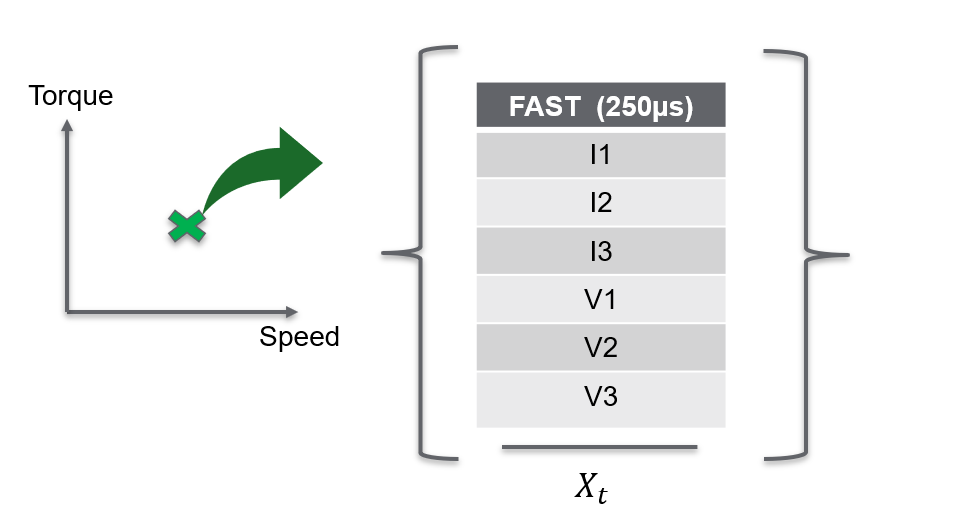
\includegraphics[width=13cm]{images_pfe/speed_couple.png}
  \caption{Variables électriques collectées pour différentes combinaisons de couple et de vitesse.}
  \label{fig:speed_couple}
\end{figure}
\FloatBarrier

La collecte des données s'effectue sur une durée de 20 secondes, avec un
échantillonnage à haute fréquence, toutes les 250 (\(\mu s\)). Ce taux
d'échantillonnage élevé permet de capturer les variations rapides et les
dynamiques transitoires du moteur, fournissant ainsi un aperçu détaillé de son
comportement électrique. Au terme de cette période de collecte, un tableau de
80 000 points de données est crée, chaque point étant enregistré de manière
chronologique pour former une série temporelle.

Par exemple, la série temporelle illustrée dans la figure \ref{fig:data_v_i}
correspond au point de fonctionnement (Couple = 0\%, Vitesse = 15\%). Cette
série est composée de 80 000 points, chaque point ayant été collecté à un
intervalle de 250 (\(\mu s\)).

\begin{figure}[hbt!]
  \centering
  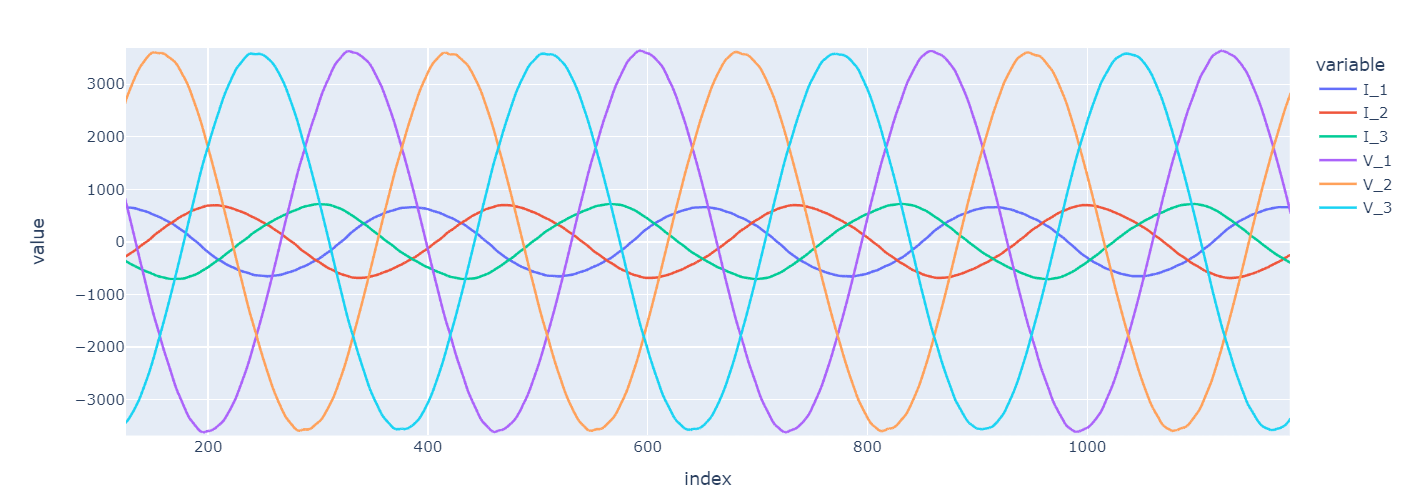
\includegraphics[width=14cm]{images_pfe/V_I_data.png}
  \caption{Signaux \((V_1, V_2, V_3, I_1, I_2, I_3)\) mesurés au point de fonctionnement \((0, 15.0)\) du moteur.}
  \label{fig:data_v_i}
\end{figure}
\FloatBarrier

À terme, notre objectif est de constituer un jeu de données exhaustif regroupant l'ensemble des points
de fonctionnement avec leurs variables électriques correspondantes. Afin d'enrichir ce jeu de données,
nous intégrons des colonnes supplémentaires représentant la vitesse, le couple, ainsi que le glissement [Figure \ref{fig:data_vcg}].
Ces nouvelles variables permettent de mieux caractériser le comportement du moteur sous diverses conditions
de fonctionnement, assurant ainsi que notre modèle génératif puisse correctement associer les variables
électriques aux combinaisons spécifiques de couple et de vitesse.

\begin{figure}[hbt!]
  \centering
  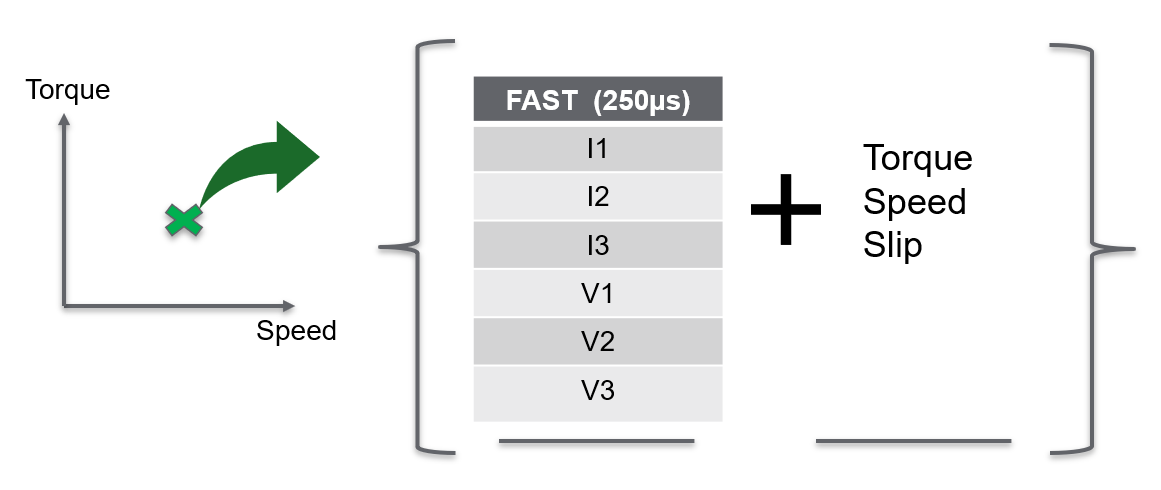
\includegraphics[width=13cm]{images_pfe/couple_vittese_glissement.png}
  \caption{Intégration des valeurs de couple, vitesse et glissement aux variables électriques dans le jeu de données d'entraînement.}
  \label{fig:data_vcg}
\end{figure}
\FloatBarrier

\subsubsection{Segmentation des Données}
Un autre défi majeur dans la génération de données est lié à la taille
considérable des séries temporelles. Par exemple, un seul point de
fonctionnement est représenté par une série temporelle composée de 80 000
points de données. Cette quantité massive de données pose des contraintes
significatives en termes de capacité de calcul et de stockage. De plus, pour
les modèles de réseaux de neurones récurrents ou autres modèles séquentiels, il
est difficile de maintenir les dépendances temporelles sur une séquence aussi
longue. En effet, un modèle qui traite un point à la position 70 000 pourrait
avoir du mal à conserver une mémoire efficace des informations importantes
présentes à la position 10, ce qui peut compromettre la qualité des
prédictions.

Pour rendre le processus plus gérable et optimiser l'apprentissage des modèles,
nous avons décidé de segmenter les séries temporelles en sous-séquences plus
courtes. Dans notre cas, nous avons choisi de segmenter les séries temporelles
en blocs de taille définie par un paramètre \texttt{seq\_len}, qui se situe
dans l'intervalle [1000, 2000]. Cette segmentation permet non seulement de
réduire la charge computationnelle, mais aussi de faciliter l'entraînement des
modèles en leur permettant de mieux capturer les relations temporelles à
l'intérieur de ces sous-séquences plus courtes. Ainsi, chaque segment conserve
une portion significative de la dynamique du moteur tout en rendant
l'apprentissage plus efficace et plus pratique.

\subsubsection{Normalisation des Données}

Les valeurs de courant et de tension mesurées dans les moteurs électriques sont
souvent très élevées, ce qui peut poser des problèmes lors de l'entraînement
des modèles de machine learning, en particulier pour les réseaux de neurones.
Afin de rendre ces valeurs plus compatibles avec les algorithmes
d'apprentissage, il est essentiel de les normaliser.

La normalisation consiste à transformer les valeurs de courant et de tension
pour les ramener dans une échelle plus réduite et uniforme. Cela présente
plusieurs avantages. Premièrement, elle permet de prévenir la domination des
valeurs de tension, qui sont généralement supérieures aux valeurs de courant.
En effet, si les valeurs de tension ne sont pas normalisées, elles peuvent
influencer de manière disproportionnée les décisions du modèle, au détriment
des valeurs de courant. En normalisant ces deux ensembles de données dans un
même intervalle, nous assurons un traitement équitable de toutes les variables
par le modèle, évitant ainsi les biais induits par des échelles de grandeur
différentes.

Deuxièmement, la normalisation facilite l'entraînement des réseaux de neurones
en accélérant leur convergence vers un minimum global ou local. Les réseaux de
neurones sont particulièrement sensibles aux échelles des données d'entrée.
Lorsque les entrées varient sur des plages de valeurs très différentes, les
gradients utilisés pour ajuster les poids des connexions peuvent devenir
instables, ralentissant ainsi le processus d'apprentissage et rendant plus
difficile la minimisation de la fonction de coût. En normalisant les données,
on obtient des gradients plus homogènes, ce qui améliore la stabilité et la
rapidité de convergence de l'algorithme d'optimisation.

Pour cela, nous avons mis en œuvre deux méthodes de normalisation : la
normalisation Min-Max et la normalisation nominale, cette dernière étant
couramment utilisée par l'équipe de Schneider Electric.

\textbf{MinMax}

La normalisation Min-Max est une technique de prétraitement des données qui
permet de redimensionner les valeurs d'une variable afin qu'elles se situent
dans un intervalle spécifique, généralement entre 0 et 1. La normalisation
Min-Max est définie par la formule suivante :

\begin{equation}
  x' = \frac{x - x_{\text{min}}}{x_{\text{max}} - x_{\text{min}}}
\end{equation}

où :

\begin{conditions}
  x & la valeur originale de la variable \\
  x_{\text{min}} &  la valeur minimale de la variable dans l'ensemble de données \\
  x_{\text{max}} &  la valeur maximale de la variable dans l'ensemble de données \\
  x' &  la valeur normalisée
\end{conditions}

Cette transformation ramène toutes les valeurs des courants et des tensions
dans l'intervalle \([0, 1]\), comme illustré dans la figure (5.5).

\begin{figure}[hbt!]
  \centering
  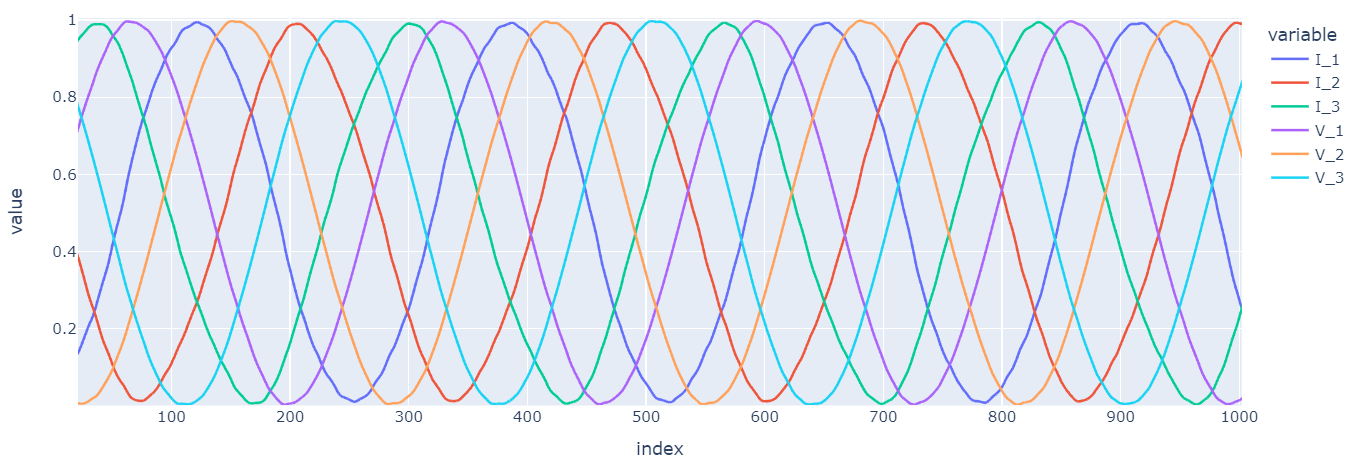
\includegraphics[width=14cm]{images_pfe/V_I_data_norm.png}
  \caption{Organization de data [\cite{yoon2019time}].}
  \label{fig:data_norm}
\end{figure}
\FloatBarrier

\textbf{Normalisation Nominale}

En utilisant la normalisation nominale, telle que proposée par l'équipe de
Schneider Electric, l'algorithme se présente comme suit :

\begin{algorithm}[H]
  \caption{Normalization Nominale}
  \KwIn{Valeurs des courants et tensions}
  \KwOut{Valeurs normalisées des courants et tensions}

  \SetKw{Initialization}{Initialisation:}
  \Initialization{}

  \( V_{\text{nom}} \gets 400 \) \;
  \( V_{\text{max}} \gets 921 \) \;
  \( I_{\text{nom}} \gets 10.2 \) \;
  \( I_{\text{max}} \gets 35.59 \) \;

  \SetKw{Normalization}{Normalisation:}
  \Normalization{}

  \( I_1 \gets I_1 \times \frac{I_{\text{max}}}{2^{12} \times I_{\text{nom}}} \) \;

  \( I_2 \gets I_2 \times \frac{I_{\text{max}}}{2^{12} \times I_{\text{nom}}} \) \;
  \( I_3 \gets I_3 \times \frac{I_{\text{max}}}{2^{12} \times I_{\text{nom}}} \) \;

  \( V_1 \gets V_1 \times \frac{V_{\text{max}}}{2^{12} \times V_{\text{nom}}} \) \;
  \( V_2 \gets V_2 \times \frac{V_{\text{max}}}{2^{12} \times V_{\text{nom}}} \) \;
  \( V_3 \gets V_3 \times \frac{V_{\text{max}}}{2^{12} \times V_{\text{nom}}} \) \;

  \KwRet{Valeurs normalisées des courants \( I_1, I_2, I_3 \) et des tensions \( V_1, V_2, V_3 \)}

\end{algorithm}
\FloatBarrier

Dans la figure suivante, nous observons les courants et tensions normalisés
avec cette technique:

\begin{figure}[hbt!]
  \centering
  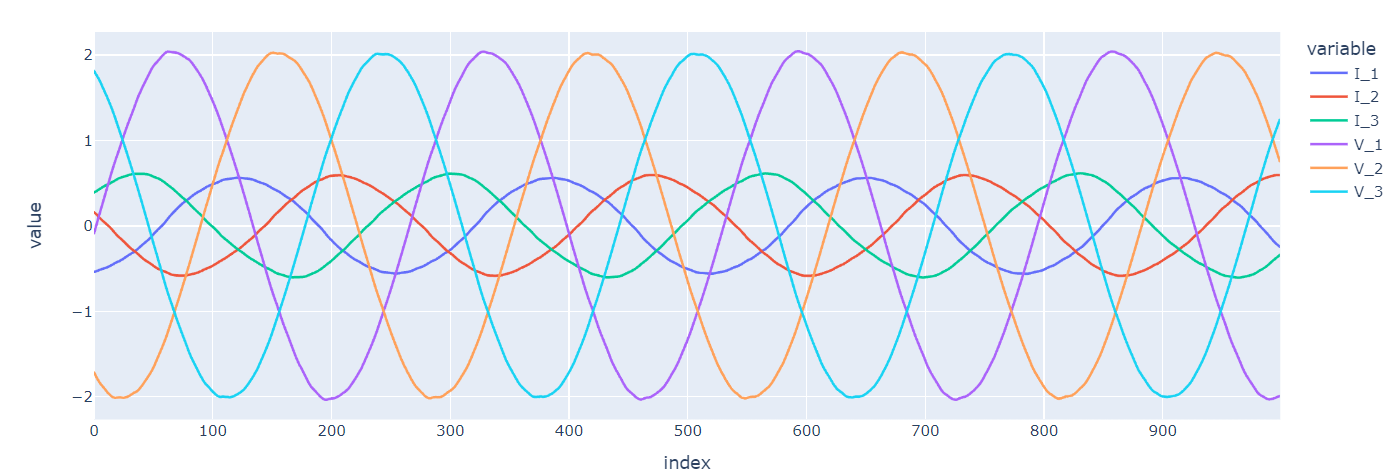
\includegraphics[width=14cm]{images_pfe/normalization_nominale.png}
  \caption{Organization de data [\cite{yoon2019time}].}
  \label{fig:data_norm}
\end{figure}
\FloatBarrier

\section{Solution proposée}

\subsection{TimeGAN}

Dans notre approche pour générer des données sous forme de séries temporelles
correspondant à celles des moteurs électriques, nous nous sommes inspirés d'un
modèle génératif nommé Time-series GAN (TimeGAN), présenté dans l'article de
  [\cite{yoon2019time}], Dans ce qui suit, nous présenterons en détail
l'architecture de notre modèle génératif, en exposant les différents composants
ainsi que les fondements théoriques sur lesquels repose notre modèle.

\subsubsection{Architecure de TimeGAN}

Compte tenu de la nature séquentielle des données utilisées, qui prennent la
forme de séries temporelles, l'architecture des réseaux de neurones adoptée
repose sur des réseaux de neurones récurrents (RNN). Afin d'améliorer les
performances du modèle, une architecture basée sur des réseaux LSTM (Long
Short-Term Memory) a été intégrée, en complément de réseaux entièrement
connectés (fully connected layers). La figure (5.7) présente l'architecture
globale du modèle génératif proposé.

Le modèle TimeGAN se structure autour de quatre réseaux de neurones principaux
: une fonction d'embedding (encodeur), une fonction de recovery (décodeur), un
générateur de séquences et un discriminateur. Ces quatre réseaux interagissent
au sein d'un espace latent une représentations réduites des données.

\textbf{Réseaux d'Embedding et de Recovery}

Les fonctions d'embedding et de recovery établissent les liens entre l'espace
des caractéristiques et l'espace latent, permettant au modèle d'apprendre les
dynamiques temporelles des données sous une forme réduite. Le réseau
d'embedding convertit les données de séries temporelles en une représentation
latente. Le réseau de recovery cherche ensuite à reconstruire la série
temporelle originale à partir de cette représentation réduite. La fonction de
perte vise à minimiser l'écart entre la série temporelle initiale et celle
reconstruite à partir de l'espace latent.

\textbf{Réseaux de Générateur et de Discriminateur}

On commence par le réseau générateur, qui prend en entrée un bruit (bruit
gaussien) et tente de générer des vecteurs dans l'espace latent, en s'assurant
que ces vecteurs se rapprochent de ceux encodés par le réseau d'embedding.
Ensuite, le discriminateur intervient en prenant en entrée les vecteurs générés
par le générateur et vérifie leur similitude avec les vecteurs originaux
encodés par le réseau de recovery. Le discriminateur guide et ajuste ainsi le
générateur, de sorte que la fonction de perte incite le générateur à produire
des vecteurs de plus en plus similaires aux vecteurs originaux.

\begin{figure}[hbt!]
  \centering
  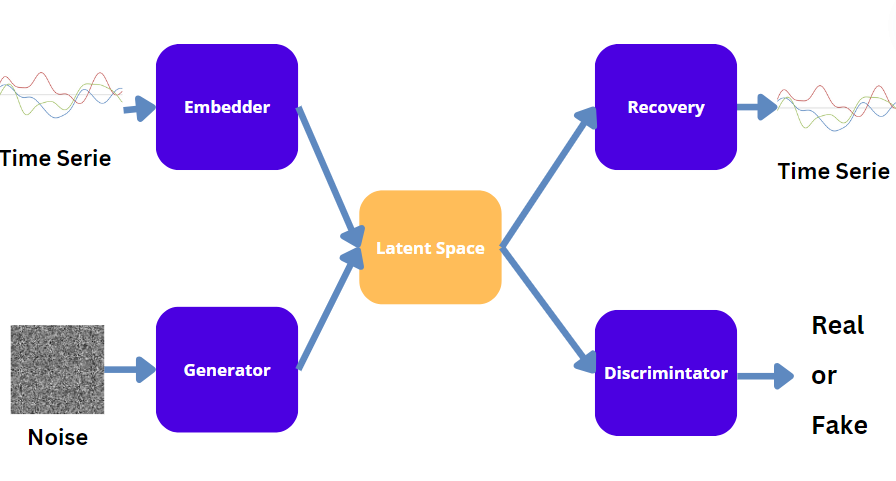
\includegraphics[width=14cm]{images_pfe/timegan_archi_.png}
  \caption{Architecure de TimeGAN[\cite{yoon2019time}].}
  \label{fig:timegan}
\end{figure}
\FloatBarrier

\textbf{Géneration de données}

Une fois que l'entraînement du modèle est terminé et que le modèle a convergé,
la génération de données devient simple. Il suffit de fournir un bruit au
réseau générateur, qui va alors produire des vecteurs dans l'espace latent. Ces
vecteurs sont ensuite décodés en séries temporelles par le réseau de recovery.

\begin{figure}[hbt!]
  \centering
  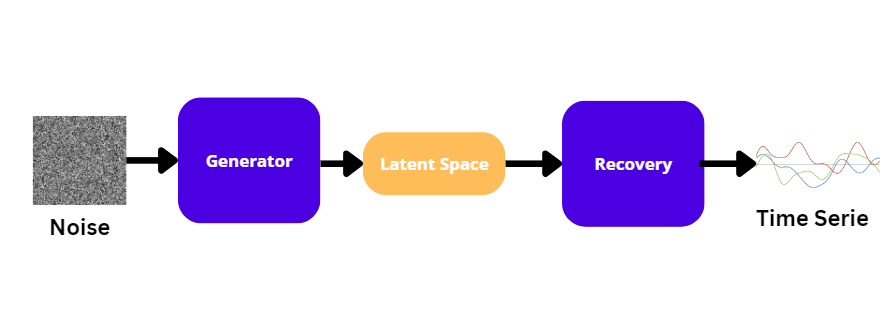
\includegraphics[width=14cm]{images_pfe/gents.png}
  \caption{Architecure de TimeGAN[\cite{yoon2019time}].}
  \label{fig:timegan}
\end{figure}
\FloatBarrier

\section{Conclusion}
Dans ce chapitre, nous avons présenté les différentes étapes suivies pour
concevoir notre méthode de génération de séries temporelles. Nous avons
détaillé l'architecture globale de notre modèle, qui se compose de quatre
réseaux de neurones : le générateur, le discriminateur, le réseau de
récupération et le réseau d'embedding. Nous avons également montré comment ces
réseaux génèrent les données et comment ils fonctionnent ensemble dans un
espace latent, utilisé pour la compression des données.

Nous avons expliqué l'organisation des jeux de données et l'importance de la
segmentation des séries temporelles. De plus, nous avons discuté des techniques
de normalisation, que ce soit avec la méthode MinMax ou avec la technique
proposée par STIE.

Dans le chapitre suivant, nous présenterons nos expérimentations sur notre
méthode pour générer des données pour des moteurs asynchrones.